% GENERATED FILE - do not hand-edit.
% Source of truth: data/calculus-reviewed/t-9.json in the zenith-website repo.
% Regenerate with: python3 scripts/build_calculus_tex.py
\documentclass[11pt]{article}
\usepackage[utf8]{inputenc}
\usepackage[T1]{fontenc}
\usepackage{amsmath,amssymb}
\usepackage{graphicx}
\usepackage[margin=1in]{geometry}
\graphicspath{{../..//}}
\setlength{\parindent}{0pt}
\setlength{\parskip}{0.6em}
\begin{document}
\section*{Chapter 9: Differential Equations --- Test T9}

\bigskip\noindent\textbf{T1.}\ Here $a$ is acceleration, $v$ velocity, and $s$ position. If $a(t)=6t-1$ and $v(2)=5$, then $v(t)$ equals
\begin{list}{}{\setlength{\leftmargin}{3em}\setlength{\labelwidth}{2.5em}\setlength{\itemsep}{0pt}\setlength{\topsep}{2pt}}
\item[(A)] $3t^2-t$
\item[(B)] $3t^2-t-5$
\item[(C)] $3t^2-t+5$
\item[(D)] $3t^2+5$
\end{list}

\bigskip\noindent\textbf{T2.}\ Here $a$ is acceleration, $v$ velocity, and $s$ position. If $a(t)=6t^2-2$, $s(-1)=1$, and $s(1)=5$, then $v(t)$ equals
\begin{list}{}{\setlength{\leftmargin}{3em}\setlength{\labelwidth}{2.5em}\setlength{\itemsep}{0pt}\setlength{\topsep}{2pt}}
\item[(A)] $2t^3-2t+2$
\item[(B)] $2t^3-2t+1$
\item[(C)] $\dfrac{t^4}{2}-t^2+2t+3.5$
\item[(D)] $\dfrac{t^4}{2}-t^2+1$
\end{list}

\bigskip\noindent\textbf{T3.}\ Here $a$ is acceleration, $v$ velocity, and $s$ position. If $a(t)=6t^2-2$, $s(-1)=1$, and $s(1)=5$, then $s(0)$ equals
\begin{list}{}{\setlength{\leftmargin}{3em}\setlength{\labelwidth}{2.5em}\setlength{\itemsep}{0pt}\setlength{\topsep}{2pt}}
\item[(A)] $2$
\item[(B)] $3$
\item[(C)] $3.5$
\item[(D)] $4$
\end{list}

\bigskip\noindent\textbf{T4.}\ A stone is thrown straight up from the top of a building with initial velocity 48 ft/sec and hits the ground 5 seconds later. The height of the building, in feet, is Use gravitational acceleration $-32$ ft/sec$^2$.
\begin{list}{}{\setlength{\leftmargin}{3em}\setlength{\labelwidth}{2.5em}\setlength{\itemsep}{0pt}\setlength{\topsep}{2pt}}
\item[(A)] $120$
\item[(B)] $140$
\item[(C)] $160$
\item[(D)] $180$
\end{list}

\bigskip\noindent\textbf{T5.}\ A stone is thrown straight up from the top of a building with initial velocity 48 ft/sec and hits the ground 5 seconds later. The maximum height is reached by the stone after Use gravitational acceleration $-32$ ft/sec$^2$.
\begin{list}{}{\setlength{\leftmargin}{3em}\setlength{\labelwidth}{2.5em}\setlength{\itemsep}{0pt}\setlength{\topsep}{2pt}}
\item[(A)] $1$ second
\item[(B)] $3/2$ seconds
\item[(C)] $2$ seconds
\item[(D)] $5/2$ seconds
\end{list}

\bigskip\noindent\textbf{T6.}\ If a car accelerates from 0 to 45 mph in 10 seconds, what distance does it travel in those 10 seconds? (Assume the acceleration is constant and note that 45 mph = 66 ft/sec.)
\begin{list}{}{\setlength{\leftmargin}{3em}\setlength{\labelwidth}{2.5em}\setlength{\itemsep}{0pt}\setlength{\topsep}{2pt}}
\item[(A)] $66$ feet
\item[(B)] $165$ feet
\item[(C)] $330$ feet
\item[(D)] $660$ feet
\end{list}

\bigskip\noindent\textbf{T7.}\ A stone is thrown at a target so that its velocity is $v(t)=120-20t$ ft/sec, where $t$ is measured in seconds. If the stone hits the target in 1 second, then the distance from the sling to the target is
\begin{list}{}{\setlength{\leftmargin}{3em}\setlength{\labelwidth}{2.5em}\setlength{\itemsep}{0pt}\setlength{\topsep}{2pt}}
\item[(A)] $90$ feet
\item[(B)] $100$ feet
\item[(C)] $110$ feet
\item[(D)] $120$ feet
\end{list}

\bigskip\noindent\textbf{T8.}\ A stone is thrown straight up from the ground. What should the initial velocity be if you want the stone to reach a height of 144 feet? Use gravitational acceleration $-32$ ft/sec$^2$.
\begin{list}{}{\setlength{\leftmargin}{3em}\setlength{\labelwidth}{2.5em}\setlength{\itemsep}{0pt}\setlength{\topsep}{2pt}}
\item[(A)] $80$ ft/sec
\item[(B)] $88$ ft/sec
\item[(C)] $96$ ft/sec
\item[(D)] $104$ ft/sec
\end{list}

\bigskip\noindent\textbf{T9.}\ If the velocity of a car traveling in a straight line at time $t$ is $v(t)$, then the difference in its odometer readings between times $t=a$ and $t=b$ is
\begin{list}{}{\setlength{\leftmargin}{3em}\setlength{\labelwidth}{2.5em}\setlength{\itemsep}{0pt}\setlength{\topsep}{2pt}}
\item[(A)] $\displaystyle\int_a^b |v(t)|\,dt$
\item[(B)] $\displaystyle\int_a^b v(t)\,dt$
\item[(C)] the net displacement of the car's position from $t=a$ to $t=b$
\item[(D)] the change in the car's position from $t=a$ to $t=b$
\end{list}

\bigskip\noindent\textbf{T10.}\ If an object is moving up and down along the $y$-axis with velocity $v(t)$ and $s'(t)=v(t)$, then it is false that $\displaystyle\int_a^b v(t)\,dt$ gives
\begin{list}{}{\setlength{\leftmargin}{3em}\setlength{\labelwidth}{2.5em}\setlength{\itemsep}{0pt}\setlength{\topsep}{2pt}}
\item[(A)] $s(b)-s(a)$
\item[(B)] the total change in $s(t)$ between $t=a$ and $t=b$
\item[(C)] the shift in the object's position from $t=a$ to $t=b$
\item[(D)] the total distance covered by the object from $t=a$ to $t=b$
\end{list}

\bigskip\noindent\textbf{T11.}\ Solutions of the differential equation $\dfrac{dy}{dx}=\dfrac{x}{4y}$ are of the form
\begin{list}{}{\setlength{\leftmargin}{3em}\setlength{\labelwidth}{2.5em}\setlength{\itemsep}{0pt}\setlength{\topsep}{2pt}}
\item[(A)] $x^2-4y^2=C$
\item[(B)] $x^2+4y^2=C$
\item[(C)] $x^2-Cy^2=0$
\item[(D)] $x^2=C-4y^2$
\end{list}

\bigskip\noindent\textbf{T12.}\ Find the domain of the particular solution to the differential equation $\dfrac{dy}{dx}=\dfrac{x}{4y}$ that passes through the point $(-3,1)$.
\begin{list}{}{\setlength{\leftmargin}{3em}\setlength{\labelwidth}{2.5em}\setlength{\itemsep}{0pt}\setlength{\topsep}{2pt}}
\item[(A)] $x<0$
\item[(B)] $-3\leq x<-\sqrt{5}$
\item[(C)] $x<-\sqrt{5}$
\item[(D)] $|x|>\sqrt{5}$
\end{list}

\bigskip\noindent\textbf{T13.}\ If $\dfrac{dy}{dx}=\dfrac{y}{3\sqrt{x}}$ and $y=1$ when $x=9$, then
\begin{list}{}{\setlength{\leftmargin}{3em}\setlength{\labelwidth}{2.5em}\setlength{\itemsep}{0pt}\setlength{\topsep}{2pt}}
\item[(A)] $\ln y = \dfrac{2}{3}\sqrt{x}-6$
\item[(B)] $\ln y = \dfrac{2}{3}\sqrt{x}-2$
\item[(C)] $y=e^{(2/3)\sqrt{x}}$
\item[(D)] $y=e^{(2/3)(\sqrt{x}-2)}$
\end{list}

\bigskip\noindent\textbf{T14.}\ If $\dfrac{dy}{dx}=e^y$ and $y=0$ when $x=2$, then
\begin{list}{}{\setlength{\leftmargin}{3em}\setlength{\labelwidth}{2.5em}\setlength{\itemsep}{0pt}\setlength{\topsep}{2pt}}
\item[(A)] $y=\ln(x)$
\item[(B)] $y=\ln(3-x)$
\item[(C)] $y=-\ln(3-x)$
\item[(D)] $y=-\ln(x)$
\end{list}

\bigskip\noindent\textbf{T15.}\ If $\dfrac{dy}{dx}=\dfrac{x}{\sqrt{16+x^2}}$ and $y=5$ when $x=3$, then $y$ equals
\begin{list}{}{\setlength{\leftmargin}{3em}\setlength{\labelwidth}{2.5em}\setlength{\itemsep}{0pt}\setlength{\topsep}{2pt}}
\item[(A)] $\sqrt{16+x^2}-5$
\item[(B)] $\sqrt{16+x^2}$
\item[(C)] $\dfrac{\sqrt{16+x^2}+5}{2}$
\item[(D)] $\dfrac{\sqrt{16+x^2}}{2}$
\end{list}

\bigskip\noindent\textbf{T16.}\ The general solution of the differential equation $2x\,dy=3y\,dx$ is a family of
\begin{list}{}{\setlength{\leftmargin}{3em}\setlength{\labelwidth}{2.5em}\setlength{\itemsep}{0pt}\setlength{\topsep}{2pt}}
\item[(A)] circles
\item[(B)] hyperbolas
\item[(C)] parabolas
\item[(D)] none of these
\end{list}

\bigskip\noindent\textbf{T17.}\ The general solution of the differential equation $\dfrac{dy}{dx}=2y$ is a family of
\begin{list}{}{\setlength{\leftmargin}{3em}\setlength{\labelwidth}{2.5em}\setlength{\itemsep}{0pt}\setlength{\topsep}{2pt}}
\item[(A)] parabolas
\item[(B)] lines
\item[(C)] ellipses
\item[(D)] exponential curves
\end{list}

\bigskip\noindent\textbf{T18.}\ A function $f(x)$ that satisfies the equations $f(x)f'(x)=x$ and $f(0)=2$ is
\begin{list}{}{\setlength{\leftmargin}{3em}\setlength{\labelwidth}{2.5em}\setlength{\itemsep}{0pt}\setlength{\topsep}{2pt}}
\item[(A)] $f(x)=\sqrt{x^2+4}$
\item[(B)] $f(x)=\sqrt{4-x^2}$
\item[(C)] $f(x)=x+2$
\item[(D)] $f(x)=e^x+1$
\end{list}

\bigskip\noindent\textbf{T19.}\ The curve that passes through the point $(1,1)$ and whose slope at any point $(x,y)$ is given by $\dfrac{dy}{dx}=\dfrac{4y}{x}$ has the equation
\begin{list}{}{\setlength{\leftmargin}{3em}\setlength{\labelwidth}{2.5em}\setlength{\itemsep}{0pt}\setlength{\topsep}{2pt}}
\item[(A)] $4x-3=y$
\item[(B)] $y^4=x$
\item[(C)] $y=x^4$
\item[(D)] $4y^3=x^3+3$
\end{list}

\bigskip\noindent\textbf{T20.}\ Find the domain of the particular solution to the differential equation $\dfrac{dy}{dx}=\dfrac{4y}{x}$ that passes through the point $(1,1)$.
\begin{list}{}{\setlength{\leftmargin}{3em}\setlength{\labelwidth}{2.5em}\setlength{\itemsep}{0pt}\setlength{\topsep}{2pt}}
\item[(A)] all real numbers
\item[(B)] $|x|\leq 1$
\item[(C)] $x\neq 0$
\item[(D)] $x>0$
\end{list}

\bigskip\noindent\textbf{T21.}\ If $\dfrac{dy}{dx}=\dfrac{k}{x}$, where $k$ is a constant, and if $y=3$ when $x=1$ and $y=6$ when $x=e$, then, when $x=2$, $y$ equals
\begin{list}{}{\setlength{\leftmargin}{3em}\setlength{\labelwidth}{2.5em}\setlength{\itemsep}{0pt}\setlength{\topsep}{2pt}}
\item[(A)] $6$
\item[(B)] $3+3\ln 2$
\item[(C)] $3\ln 2$
\item[(D)] $6\ln 2$
\end{list}

\bigskip\noindent\textbf{T22.}\ The slope field shown below is for the differential equation
\begin{center}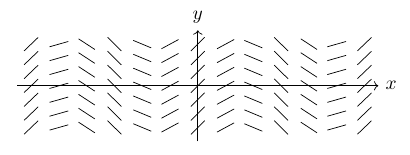
\includegraphics[width=0.6\linewidth]{data/calculus-figures/t9-t22.png}\end{center}
\begin{list}{}{\setlength{\leftmargin}{3em}\setlength{\labelwidth}{2.5em}\setlength{\itemsep}{0pt}\setlength{\topsep}{2pt}}
\item[(A)] $\dfrac{dy}{dx}=\sin x$
\item[(B)] $\dfrac{dy}{dx}=-\sin x$
\item[(C)] $\dfrac{dy}{dx}=\cos x$
\item[(D)] $\dfrac{dy}{dx}=-\cos x$
\end{list}

\bigskip\noindent\textbf{T23.}\ The slope field shown below is for the differential equation
\begin{center}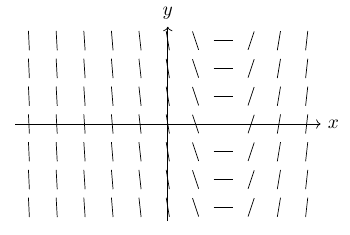
\includegraphics[width=0.6\linewidth]{data/calculus-figures/t9-t23.png}\end{center}
\begin{list}{}{\setlength{\leftmargin}{3em}\setlength{\labelwidth}{2.5em}\setlength{\itemsep}{0pt}\setlength{\topsep}{2pt}}
\item[(A)] $\dfrac{dy}{dx}=3x$
\item[(B)] $\dfrac{dy}{dx}=3x-6$
\item[(C)] $\dfrac{dy}{dx}=6-3x$
\item[(D)] $\dfrac{dy}{dx}=y$
\end{list}

\bigskip\noindent\textbf{T24.}\ A solution curve has been superimposed on the slope field shown above. The solution is for the differential equation and initial condition
\begin{center}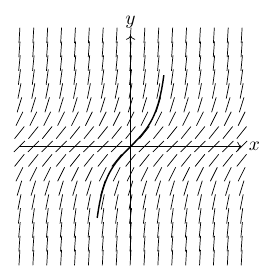
\includegraphics[width=0.6\linewidth]{data/calculus-figures/t9-t24.png}\end{center}
\begin{list}{}{\setlength{\leftmargin}{3em}\setlength{\labelwidth}{2.5em}\setlength{\itemsep}{0pt}\setlength{\topsep}{2pt}}
\item[(A)] $\dfrac{dy}{dx}=\tan x$; $y(0)=0$
\item[(B)] $\dfrac{dy}{dx}=1+x^2$; $y(0)=0$
\item[(C)] $\dfrac{dy}{dx}=\dfrac{1}{1+x^2}$; $y\left(\dfrac{\pi}{4}\right)=1$
\item[(D)] $\dfrac{dy}{dx}=1+y^2$; $y(0)=0$
\end{list}

\bigskip\noindent\textbf{T25.}\ Which slope field is for the differential equation $\dfrac{dy}{dx}=2y$?
\begin{center}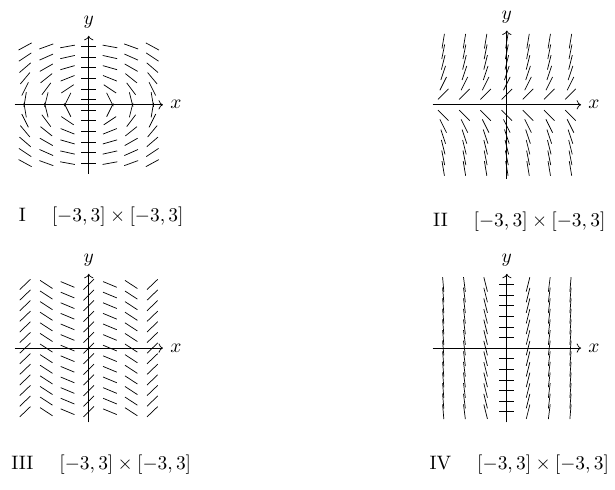
\includegraphics[width=0.6\linewidth]{data/calculus-figures/t9-t25.png}\end{center}
\begin{list}{}{\setlength{\leftmargin}{3em}\setlength{\labelwidth}{2.5em}\setlength{\itemsep}{0pt}\setlength{\topsep}{2pt}}
\item[(A)] I
\item[(B)] II
\item[(C)] III
\item[(D)] IV
\end{list}

\bigskip\noindent\textbf{T26.}\ Which slope field is for the differential equation $\dfrac{dy}{dx}=-\dfrac{x}{2y}$?
\begin{center}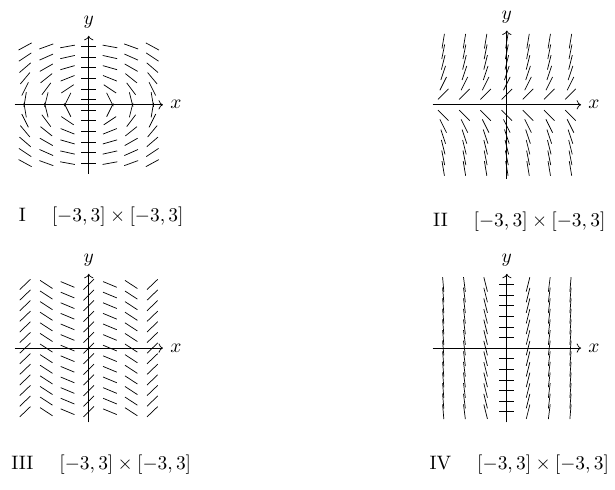
\includegraphics[width=0.6\linewidth]{data/calculus-figures/t9-t25.png}\end{center}
\begin{list}{}{\setlength{\leftmargin}{3em}\setlength{\labelwidth}{2.5em}\setlength{\itemsep}{0pt}\setlength{\topsep}{2pt}}
\item[(A)] I
\item[(B)] II
\item[(C)] III
\item[(D)] IV
\end{list}

\bigskip\noindent\textbf{T27.}\ Which slope field is for the differential equation $\dfrac{dy}{dx}=\cos 2x$?
\begin{center}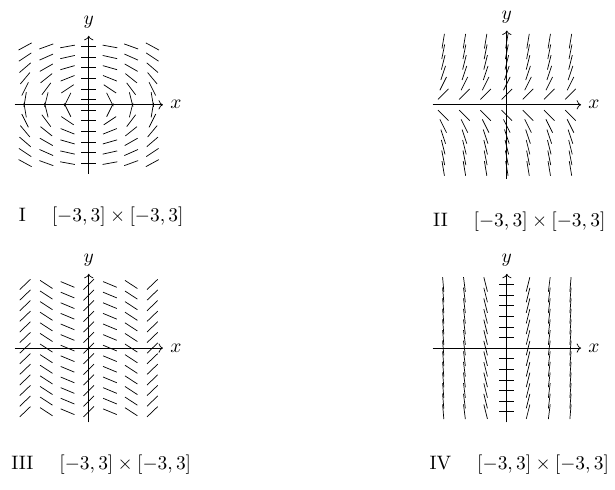
\includegraphics[width=0.6\linewidth]{data/calculus-figures/t9-t25.png}\end{center}
\begin{list}{}{\setlength{\leftmargin}{3em}\setlength{\labelwidth}{2.5em}\setlength{\itemsep}{0pt}\setlength{\topsep}{2pt}}
\item[(A)] I
\item[(B)] II
\item[(C)] III
\item[(D)] IV
\end{list}

\bigskip\noindent\textbf{T28.}\ Which slope field is for the differential equation $\dfrac{dy}{dx}=4x$?
\begin{center}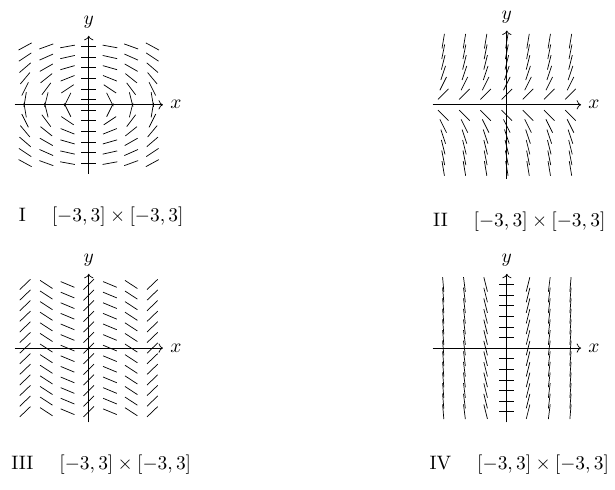
\includegraphics[width=0.6\linewidth]{data/calculus-figures/t9-t25.png}\end{center}
\begin{list}{}{\setlength{\leftmargin}{3em}\setlength{\labelwidth}{2.5em}\setlength{\itemsep}{0pt}\setlength{\topsep}{2pt}}
\item[(A)] I
\item[(B)] II
\item[(C)] III
\item[(D)] IV
\end{list}

\bigskip\noindent\textbf{T29.}\ A particular solution curve of a differential equation whose slope field is shown in II passes through the point $(0,-2)$. The equation is
\begin{center}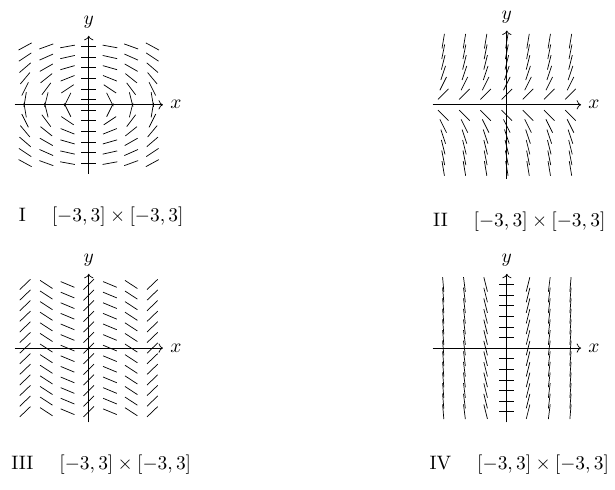
\includegraphics[width=0.6\linewidth]{data/calculus-figures/t9-t25.png}\end{center}
\begin{list}{}{\setlength{\leftmargin}{3em}\setlength{\labelwidth}{2.5em}\setlength{\itemsep}{0pt}\setlength{\topsep}{2pt}}
\item[(A)] $y=-2e^{2x}$
\item[(B)] $y=-2e^{-2x}$
\item[(C)] $y=2x^2-2$
\item[(D)] $y=-2\cos(2x)$
\end{list}

\bigskip\noindent\textbf{T30.}\ If you use Euler's method with $\Delta x = 0.15$ for the d.e.\ $\dfrac{dy}{dx}=x$, with initial value $y(1)=6$, then, when $x=1.3$, $y$ is approximately
\begin{list}{}{\setlength{\leftmargin}{3em}\setlength{\labelwidth}{2.5em}\setlength{\itemsep}{0pt}\setlength{\topsep}{2pt}}
\item[(A)] $6.10$
\item[(B)] $6.32$
\item[(C)] $6.35$
\item[(D)] $7.20$
\end{list}

\bigskip\noindent\textbf{T31.}\ For $y'=x$, $y(1)=6$, Euler's method with step $0.15$ estimates $y(1.3)$. What is the absolute error of the unrounded Euler estimate?
\begin{list}{}{\setlength{\leftmargin}{3em}\setlength{\labelwidth}{2.5em}\setlength{\itemsep}{0pt}\setlength{\topsep}{2pt}}
\item[(A)] $0.0025$
\item[(B)] $0.0125$
\item[(C)] $0.0225$
\item[(D)] $0.225$
\end{list}

\bigskip\noindent\textbf{T32.}\ Which differential equation has the slope field shown?
\begin{center}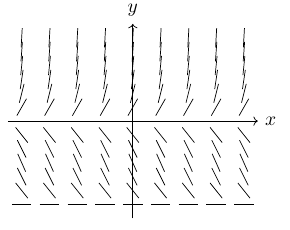
\includegraphics[width=0.6\linewidth]{data/calculus-figures/t9-t32.png}\end{center}
\begin{list}{}{\setlength{\leftmargin}{3em}\setlength{\labelwidth}{2.5em}\setlength{\itemsep}{0pt}\setlength{\topsep}{2pt}}
\item[(A)] $\dfrac{dy}{dx}=y(y+3)$
\item[(B)] $\dfrac{dy}{dx}=xy+3$
\item[(C)] $\dfrac{dy}{dx}=\dfrac{x}{y+3}$
\item[(D)] $\dfrac{dy}{dx}=\dfrac{y}{y+3}$
\end{list}

\bigskip\noindent\textbf{T33.}\ Which function is a possible solution of the slope field shown?
\begin{center}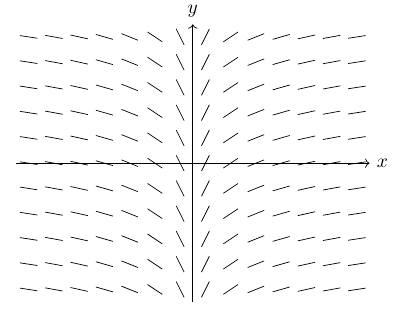
\includegraphics[width=0.6\linewidth]{data/calculus-figures/t9-t33.png}\end{center}
\begin{list}{}{\setlength{\leftmargin}{3em}\setlength{\labelwidth}{2.5em}\setlength{\itemsep}{0pt}\setlength{\topsep}{2pt}}
\item[(A)] $y=2-\ln x$
\item[(B)] $y=2+\ln x$
\item[(C)] $y=2+e^x$
\item[(D)] $y=2+\tan x$
\end{list}

\bigskip\noindent\textbf{T34.}\ Which differential equation has the slope field shown? Domain: $[-10,10]\times[-7,7]$.
\begin{center}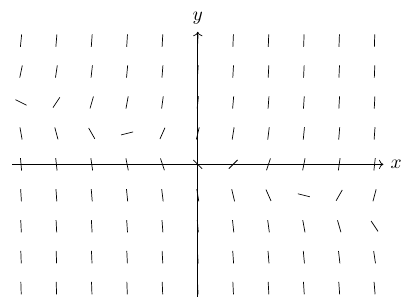
\includegraphics[width=0.6\linewidth]{data/calculus-figures/t9-t34.png}\end{center}
\begin{list}{}{\setlength{\leftmargin}{3em}\setlength{\labelwidth}{2.5em}\setlength{\itemsep}{0pt}\setlength{\topsep}{2pt}}
\item[(A)] $\dfrac{dy}{dx}=x^2+3y^2+1$
\item[(B)] $\dfrac{dy}{dx}=3y-1$
\item[(C)] $\dfrac{dy}{dx}=x-3y-1$
\item[(D)] $\dfrac{dy}{dx}=x+3y-1$
\end{list}

\bigskip\noindent\textbf{T35.}\ Which differential equation has the slope field shown? Domain: $[-10,10]\times[-7,7]$.
\begin{center}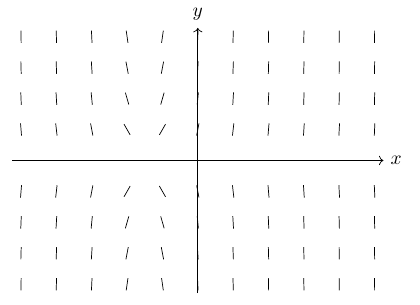
\includegraphics[width=0.6\linewidth]{data/calculus-figures/t9-t35.png}\end{center}
\begin{list}{}{\setlength{\leftmargin}{3em}\setlength{\labelwidth}{2.5em}\setlength{\itemsep}{0pt}\setlength{\topsep}{2pt}}
\item[(A)] $\dfrac{dy}{dx}=x(x+y)$
\item[(B)] $\dfrac{dy}{dx}=y(x+3)$
\item[(C)] $\dfrac{dy}{dx}=x(x+1)$
\item[(D)] $\dfrac{dy}{dx}=x(x^2+y)$
\end{list}

\bigskip\noindent\textbf{T36.}\ Which differential equation has the slope field shown? Domain: $[-10,10]\times[-4,4]$.
\begin{center}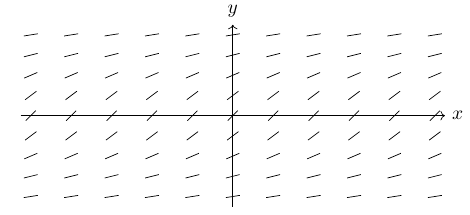
\includegraphics[width=0.6\linewidth]{data/calculus-figures/t9-t36.png}\end{center}
\begin{list}{}{\setlength{\leftmargin}{3em}\setlength{\labelwidth}{2.5em}\setlength{\itemsep}{0pt}\setlength{\topsep}{2pt}}
\item[(A)] $\dfrac{dy}{dx}=\dfrac{3x}{3+y^2}$
\item[(B)] $\dfrac{dy}{dx}=\dfrac{3}{3+x^2}$
\item[(C)] $\dfrac{dy}{dx}=\dfrac{3y}{3+y^2}$
\item[(D)] $\dfrac{dy}{dx}=\dfrac{3}{3+y^2}$
\end{list}

\bigskip\noindent\textbf{TB1.}\ If $\dfrac{ds}{dt}=\sin^2\left(\dfrac{\pi}{3}s\right)$ and if $s=1$ when $t=0$, then, when $s=2$, $t$ is equal to
\begin{list}{}{\setlength{\leftmargin}{3em}\setlength{\labelwidth}{2.5em}\setlength{\itemsep}{0pt}\setlength{\topsep}{2pt}}
\item[(A)] $\dfrac{1}{2}$
\item[(B)] $\dfrac{\sqrt{3}}{2}$
\item[(C)] $\dfrac{2\sqrt{3}}{\pi}$
\item[(D)] $-\dfrac{2\sqrt{3}}{\pi}$
\end{list}

\bigskip\noindent\textbf{TB2.}\ If radium decomposes at a rate proportional to the amount present, then the amount $R$ left after $t$ years, if $R_0$ is present initially and $k$ is the negative constant of proportionality, is given by
\begin{list}{}{\setlength{\leftmargin}{3em}\setlength{\labelwidth}{2.5em}\setlength{\itemsep}{0pt}\setlength{\topsep}{2pt}}
\item[(A)] $R=R_0 kt$
\item[(B)] $R=R_0 e^{kt}$
\item[(C)] $R=e^{R_0 kt}$
\item[(D)] $R=e^{R_0+kt}$
\end{list}

\bigskip\noindent\textbf{TB3.}\ The population of a city increases continuously at a rate proportional, at any time, to the population at that time. The population doubles in 30 years. After 75 years the ratio of the population $P$ to the initial population $P_0$ is
\begin{list}{}{\setlength{\leftmargin}{3em}\setlength{\labelwidth}{2.5em}\setlength{\itemsep}{0pt}\setlength{\topsep}{2pt}}
\item[(A)] $\dfrac{9}{4}$
\item[(B)] $\dfrac{5}{2}$
\item[(C)] $4\sqrt{2}$
\item[(D)] $\dfrac{4}{1}$
\end{list}

\bigskip\noindent\textbf{TB4.}\ If a substance decomposes at a rate proportional to the amount of the substance present, and if the amount decreases from 80 g to 20 g in 4 hours, then the constant of proportionality is
\begin{list}{}{\setlength{\leftmargin}{3em}\setlength{\labelwidth}{2.5em}\setlength{\itemsep}{0pt}\setlength{\topsep}{2pt}}
\item[(A)] $-\ln 2$
\item[(B)] $-\dfrac{\ln 2}{2}$
\item[(C)] $-\dfrac{1}{4}$
\item[(D)] $\ln\dfrac{1}{4}$
\end{list}

\bigskip\noindent\textbf{TB5.}\ If $(g'(x))^2=g(x)$ for all real $x$ and $g(0)=0$, $g(6)=9$, then $g(2)$ equals
\begin{list}{}{\setlength{\leftmargin}{3em}\setlength{\labelwidth}{2.5em}\setlength{\itemsep}{0pt}\setlength{\topsep}{2pt}}
\item[(A)] $\dfrac{1}{4}$
\item[(B)] $\dfrac{1}{2}$
\item[(C)] $1$
\item[(D)] $4$
\end{list}

\bigskip\noindent\textbf{TB6.}\ The solution curve of $\dfrac{dy}{dx}=2y$ that passes through point $(1,5)$ is
\begin{list}{}{\setlength{\leftmargin}{3em}\setlength{\labelwidth}{2.5em}\setlength{\itemsep}{0pt}\setlength{\topsep}{2pt}}
\item[(A)] $y=e^{2x}+5$
\item[(B)] $y=0.677e^{2x}$
\item[(C)] $y=e^{2x}-(e^2+5)$
\item[(D)] $y=e^{2x}/0.677$
\end{list}

\bigskip\noindent\textbf{TB7.}\ At any point of intersection of a solution curve of the d.e.\ $\dfrac{dy}{dx}=x+2y$ and the line $x+2y=0$, the function $y$ at that point
\begin{list}{}{\setlength{\leftmargin}{3em}\setlength{\labelwidth}{2.5em}\setlength{\itemsep}{0pt}\setlength{\topsep}{2pt}}
\item[(A)] is equal to $0$
\item[(B)] is a local maximum
\item[(C)] is a local minimum
\item[(D)] has a point of inflection
\end{list}

\bigskip\noindent\textbf{TB8.}\ If $F\prime(x)=2e^{-2x^2}$ and $F(0)=0$, find $\lim_{x\to\infty}F(x)$ to three decimal places.
\begin{list}{}{\setlength{\leftmargin}{3em}\setlength{\labelwidth}{2.5em}\setlength{\itemsep}{0pt}\setlength{\topsep}{2pt}}
\item[(A)] $1.253$
\item[(B)] $1.772$
\item[(C)] $2.000$
\item[(D)] $\infty$
\end{list}

\bigskip\noindent\textbf{TB9.}\ The graph displays logistic growth for a frog population $F$, with limiting value 1500. Which differential equation could be the appropriate model?
\begin{center}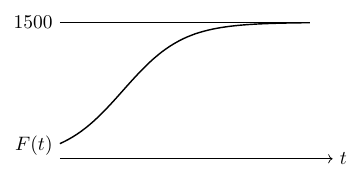
\includegraphics[width=0.6\linewidth]{data/calculus-figures/t9-tb9.png}\end{center}
\begin{list}{}{\setlength{\leftmargin}{3em}\setlength{\labelwidth}{2.5em}\setlength{\itemsep}{0pt}\setlength{\topsep}{2pt}}
\item[(A)] $\dfrac{dF}{dt}=3F-0.002F^2$
\item[(B)] $\dfrac{dF}{dt}=4F^2-0.002F$
\item[(C)] $\dfrac{dF}{dt}=4F-0.002F^2$
\item[(D)] $\dfrac{dF}{dt}=0.002F^2-4F$
\end{list}

\bigskip\noindent\textbf{TB10.}\ The derivative table is $\begin{array}{c|rrrrrr}x&3&5&7&9&11&13\\\hline f\prime(x)&2.5&3&1.5&-1&-2&1\end{array}$. Given $f(3)=120$, use Euler\'s method with step size $2$ to estimate $f(9)$.
\begin{list}{}{\setlength{\leftmargin}{3em}\setlength{\labelwidth}{2.5em}\setlength{\itemsep}{0pt}\setlength{\topsep}{2pt}}
\item[(A)] $130$
\item[(B)] $132$
\item[(C)] $134$
\item[(D)] $136$
\end{list}

\bigskip\noindent\textbf{TB11.}\ A cup of coffee at temperature $200^\circ$F is placed on a table in a room at $60^\circ$F. The d.e.\ for its temperature at time $t$ (in minutes) is $\dfrac{dy}{dt}=-0.12(y-60)$; $y(0)=200$. After 12 minutes, the temperature (in $^\circ$F) of the coffee is approximately
\begin{list}{}{\setlength{\leftmargin}{3em}\setlength{\labelwidth}{2.5em}\setlength{\itemsep}{0pt}\setlength{\topsep}{2pt}}
\item[(A)] $88$
\item[(B)] $93$
\item[(C)] $98$
\item[(D)] $105$
\end{list}

\bigskip\noindent\textbf{TB12.}\ A cup of coffee at temperature $200^\circ$F is placed on a table in a room at $60^\circ$F. The d.e.\ for its temperature at time $t$ (in minutes) is $\dfrac{dy}{dt}=-0.12(y-60)$; $y(0)=200$. Approximately how long does it take the temperature of the coffee to drop to $70^\circ$F?
\begin{list}{}{\setlength{\leftmargin}{3em}\setlength{\labelwidth}{2.5em}\setlength{\itemsep}{0pt}\setlength{\topsep}{2pt}}
\item[(A)] $18$ minutes
\item[(B)] $20$ minutes
\item[(C)] $22$ minutes
\item[(D)] $25$ minutes
\end{list}

\bigskip\noindent\textbf{TB13.}\ A medication concentration satisfies $C\prime(t)=-0.25C(t)$, with $t$ in hours and $C(0)>0$. Approximately how many hours are required for it to reach one-tenth of its initial concentration?
\begin{list}{}{\setlength{\leftmargin}{3em}\setlength{\labelwidth}{2.5em}\setlength{\itemsep}{0pt}\setlength{\topsep}{2pt}}
\item[(A)] $3$
\item[(B)] $5\dfrac{1}{3}$
\item[(C)] $8$
\item[(D)] $9.210$
\end{list}

\bigskip\noindent\textbf{TB14.}\ Which of the following statements characterize(s) the logistic growth of a population whose limiting value is $L$ and whose initial value is less than $\dfrac{L}{2}$?

 I. The growth rate initially increases. II. The growth rate is maximal at population $L/2$. III. The growth rate tends to zero as population tends to $L$.
\begin{list}{}{\setlength{\leftmargin}{3em}\setlength{\labelwidth}{2.5em}\setlength{\itemsep}{0pt}\setlength{\topsep}{2pt}}
\item[(A)] I only
\item[(B)] I and II only
\item[(C)] II and III only
\item[(D)] I, II, and III
\end{list}

\bigskip\noindent\textbf{TB15.}\ Which of the following differential equations is not logistic?
\begin{list}{}{\setlength{\leftmargin}{3em}\setlength{\labelwidth}{2.5em}\setlength{\itemsep}{0pt}\setlength{\topsep}{2pt}}
\item[(A)] $P'=P-P^2$
\item[(B)] $\dfrac{dy}{dt}=0.02y(80-y)$
\item[(C)] $\dfrac{dx}{dt}=0.6x-0.003x^2$
\item[(D)] $\dfrac{dR}{dt}=0.2(500-R)$
\end{list}

\bigskip\noindent\textbf{TB16.}\ Suppose $P(t)$ denotes the size of an animal population at time $t$ and its growth is described by the d.e.\ $\dfrac{dP}{dt}=0.003P(1500-P)$. If the initial population is 300, then the population is growing fastest
\begin{list}{}{\setlength{\leftmargin}{3em}\setlength{\labelwidth}{2.5em}\setlength{\itemsep}{0pt}\setlength{\topsep}{2pt}}
\item[(A)] initially
\item[(B)] when $P=750$
\item[(C)] when $P=1500$
\item[(D)] when $\dfrac{d^2P}{dt^2}>0$
\end{list}

\end{document}
